\documentclass[utf8]{frontiers_suppmat} % for all articles
\usepackage{url, hyperref,lineno,microtype,subcaption}
\usepackage[onehalfspacing]{setspace}
\usepackage{booktabs}
\usepackage{natbib}
\linenumbers
\usepackage{listings}

\def\keyFont{\fontsize{8}{11}\helveticabold }
\def\firstAuthorLast{Robles-Fernandez and Lira-Noriega} 
\def\Authors{Angel L. Robles-Fernandez\, Andres Lira-Noriega\ $*$}

\def\corrAuthor{Corresponding Author}
\def\corrEmail{aliranoriega@gmail.com}


\begin{document}
\onecolumn
\firstpage{1}

\title[Supplementary Material]{{\helveticaitalic{Supplementary Material}}:
\\ \helvetica{Combining phylogenetic and occurrence information for risk assessment of pest and pathogen interactions with host plants}} %Please insert the title of your article here
\author[\firstAuthorLast ]{\Authors} 
\correspondance{} 
\extraAuth{}
\maketitle

\section{Supplementary Figures}

\begin{figure}[h!]
\begin{center}
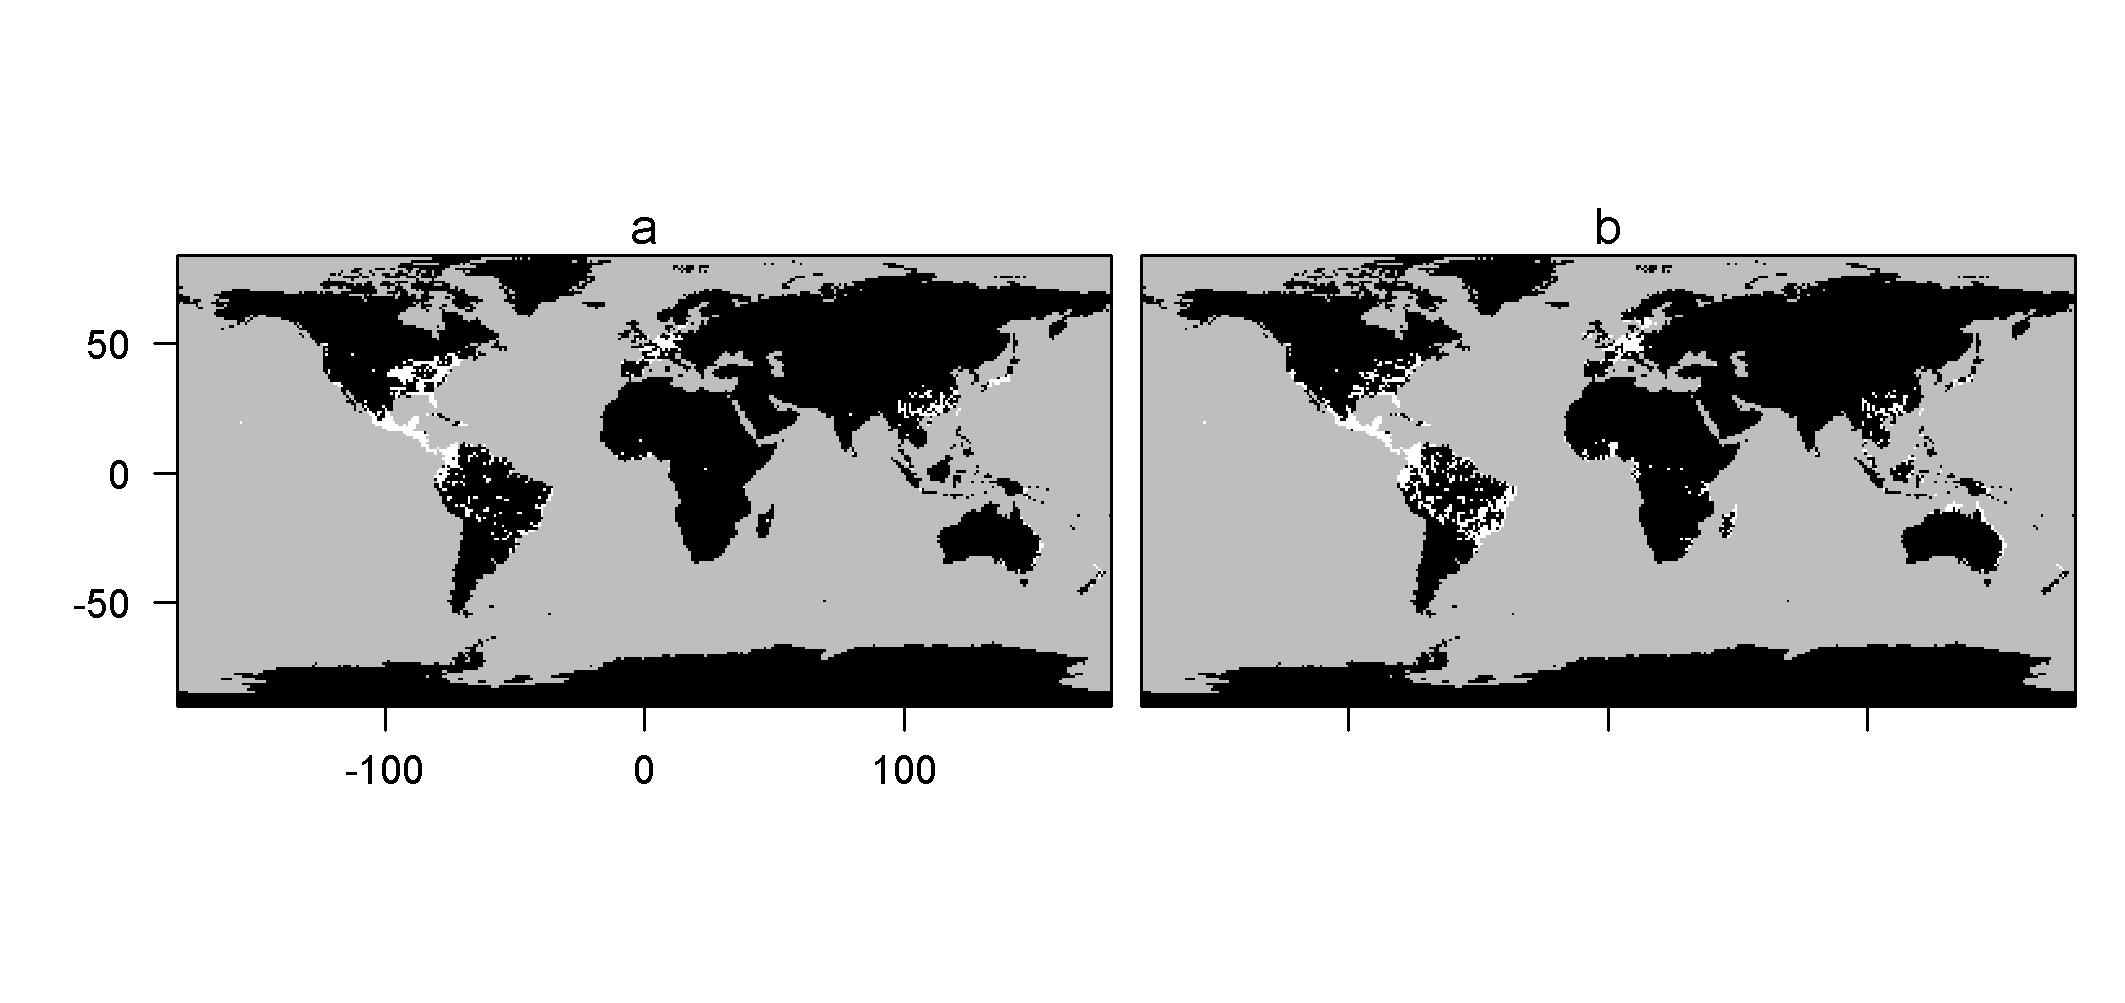
\includegraphics[width=15cm]{S1}% This is a *.jpg file
\end{center}
\caption{Interaction-or-infection spatial index and risk binary maps for $\mathbf{M_1}$ (a) and $\mathbf{M_2}$ (b) in logistic scale with values over 0.5. Maps summarize information at 1-degree spatial resolution. } \label{fig:1}
\end{figure}

\begin{figure}[h!]
\begin{center}
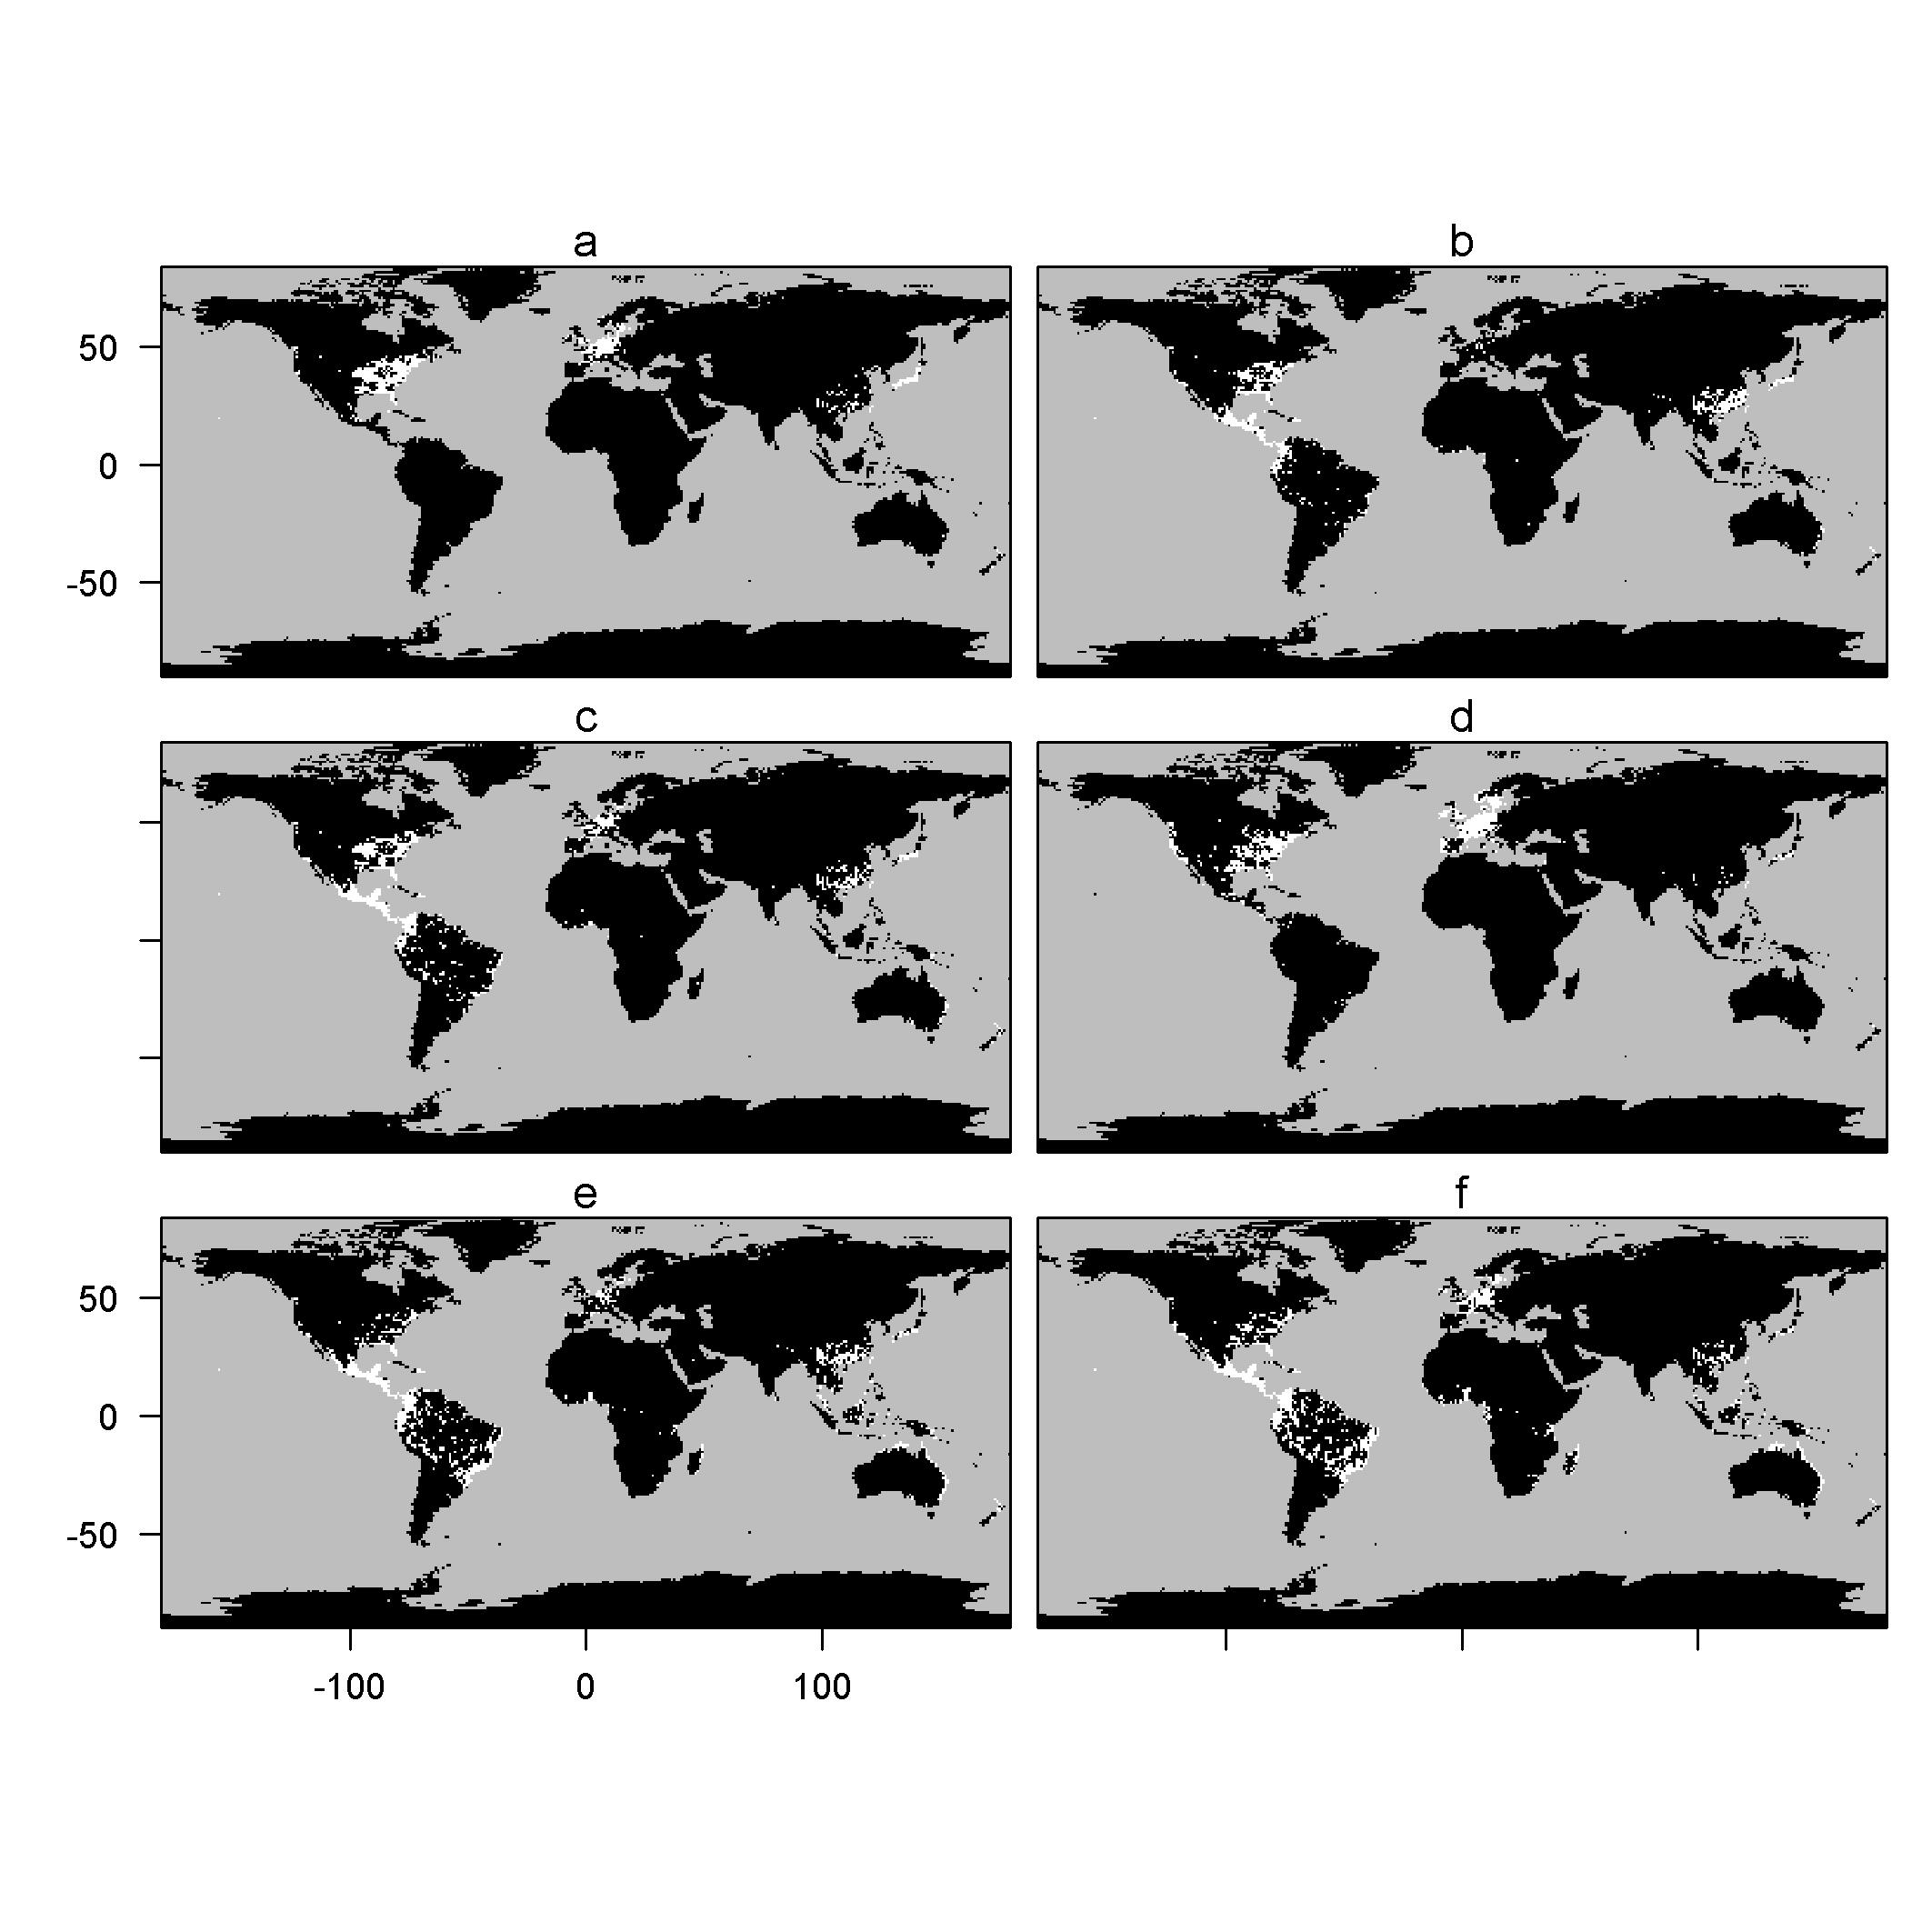
\includegraphics[width=15cm]{S2}% This is a *.jpg file
\end{center}

\caption{Spatial interaction-or-infection index binary raster in logistic scale with values over 0.5, for three cases of host range size and different level of phylogenetic constraint. Maps in a, c and e correspond to the interaction-or-infection index for host plant genera from the original host-beetle database ($\mathbf{M_1}$), and maps in b, d, and f correspond to the interaction-or-infection index for host plant genera from the phylogenetic tree ($\mathbf{M_2}$). The three cases correspond to a narrow host range phylogenetically constrained species (\textit{Xyleborus xylographus}), a wide host range vector phylogenetically constrained species (\textit{Xyleborus glabratus}), and a wide host range phylogenetically dispersed species (\textit{Xylosandrus crassiusculus}). Maps summarize information at 1-degree spatial resolution. }\label{fig:2}
\end{figure}


\clearpage

\section{R code}

\subsection{Introduction}

All the results in the article were calculated using R package geotax available through GitHub \footnote{\url{https://github.com/alrobles/geotax}}. This package contains tools to spatialize biodiveristy information over geographic space. R code file and supplies to run the code are attached as supplementary zip file and also are available in the GitHub package repository. Suggestions are welcome. 

The code needs the follow files: 

\begin{itemize}
	\item full\_ taxa\_ beetle\_ plant.csv (contains interaction information as table)
	\item M1.csv (presence-absence matrix of host by sites)
	\item M2.csv (presence-absence matrix of host by sites)
	\item m1\_ pts.csv (host presence points)
	\item m2\_ pts.csv (host presence points) and
	\item host.tree.tre (host phylogenetic tree)

\end{itemize}

Briefly, the code reads a phylogenetic tree to get the distance $\mathbf{D}$. Then reads the interaction table to convert it in $\mathbf{I}$ interaction matrix. Next it performs the logistic regression to obtain coefficients $\beta_0$ and $\beta_1$. Using these coefficients it transforms $\mathbf{D}$ in $\mathbf{P}$. After this it reads $\mathbf{M_1}$ and $\mathbf{M_2}$ matrices and using $\mathbf{P}$ and $\mathbf{M}$ gets $\mathbf{G}$ for each case (matrix). Finally, it correlates the row sums of $\mathbf{G}$ and $\mathbf{M_{1,2}}$ and obtains the linear regression between correlation coefficients and host range (number of host) $H$. The code uses non-standard evaluation syntax with use of magrittr package pipe.


\begin{lstlisting}[language=R]

#Support material
#path the the material directory
setwd("~/material")

devtools::install_github("alrobles/geotax")
require(geotax)

pack <- c("caper","phytools","geiger",
          "dismo","randomForest","SDMTools")

lapply(pack, install.packages)
lapply(pack, require, character.only = TRUE)
  
####host phylogenetical tree build with phylomatic
tree <- read.tree("host.tree")

#distance matrix
d <- tree %>% cophenetic.phylo()
d <- log10(d+1)

#not run
#d <- log10(phy_dist + 1) # using data object

#############################################
# create incidence matrix from database     #
# and filter with distance matrix           #
#############################################

db <- read.csv("full_taxa_beetle_plant.csv", header = T)
i_matrix <- incidence(db[, c(7, 13)])[ ,colnames(d)]


# filtering incidence matrix with incidence > 2
i <- i_matrix[rowSums(i_matrix)>2, ]

# distance matrix

#logistic regression coefficients for all the set
coef <- log_reg_boostrap(i, d, 1000)

#logistic regression coefficients for each case
coef_all <-  sapply(1:nrow(i),
			 function(x) log_reg_boostrap(i[x, ,drop=F], d, 1000) ) %>% t

#filter matrix for each case taking only source infected host to all target host
d_all <- lapply(1:nrow(i), function(x){ d[which(i[x, ]  %in% 1), ] })
names(d_all) <-  rownames(i)

#probability matrix for all set
p <- prob_logit(coef[c(1,7)], d)

#probability matrix for each case
p_all <- lapply(1:nrow(coef_all),
                function(x) prob_logit(coef_all[x, c(1,7)], d_all[[x]]) )
names(p_all) <- rownames(i)

#points database retrived from gbif by species data base
m1_db <- read.csv("m1_pts.csv") 

#points database retrived from gbif by genera data base
m2_db <- read.csv("m2_pts.csv") 

#presense-absence matrix from m1_db at 1 degree resolution
M1 <-  read.csv("M1.csv")   
row.names(M1) <-  M1[ ,1]
M1 <- M1[ ,-1]

##presense-absence matrix from m1_db 1 degree resolution
M2 <-  read.csv("M2.csv")   
row.names(M2) <-  M2[ ,1]
M2 <- M2[ ,-1]

#M1 and M2 can be build with geotax::PAM() with geotax::world shape

#match data from genera in points databases and probability matrix

n1 <- colnames(p)[ unique(m1_db[ ,1]) %>% as.matrix %>%
                     match(., colnames(p)) %>% na.omit ]
n2 <- colnames(p)[ unique(m2_db[ ,1]) %>% as.matrix %>%
                     match(., colnames(p)) %>% na.omit ]

#presence-absence matrix M1 and M2 filter with match
M1 <- M1[n1, ] %>% as.matrix  
M2 <- M2[n2, ] %>% as.matrix  

#probability matrix with filter
p_all_m1 <- lapply(p_all, function(x) x[, n1] ) 
p_all_m2 <- lapply(p_all, function(x) x[, n2] ) 

p_m1 <- p[n1, n1]
p_m2 <- p[n2, n2]

#calculate geographical phylogenetical information

#full set case
G1 <- p_m1 %*% M1
G2 <- p_m2 %*% M2

#all single case G matrix
G1_all <- lapply(p_all_m1, function(x) x %*% M1) 
G2_all <- lapply(p_all_m2, function(x) x %*% M2)

g1 <- richness_PAM(world, G1, 1 ) #g raster
g1_log <- 1 - g1 %>% normalize() %>% cumulative() %>% logistic()

g2 <- richness_PAM(world, G2, 1 )
g2_log <- 1 - g2 %>% normalize() %>% cumulative() %>% logistic()

g1_all <-  lapply(G1_all, function(x) richness_PAM(world, x, 1 ) )
g2_all <-  lapply(G2_all, function(x) richness_PAM(world, x, 1 ) )

#g raster in logistic scale
g1_log_all <- lapply(g1_all, function(x){
  1 - x %>% normalize() %>% cumulative() %>% logistic() } )
g2_log_all <- lapply(g2_all, function(x){
  1 - x %>% normalize() %>% cumulative() %>% logistic() } )

#richnes from M1 and M2 as raster
richness_M1 <- richness_PAM(world, M1, 1 )
richness_M2 <- richness_PAM(world, M2, 1 )


#correlation between g and M for both cases
cor_r_g1_M1 <- lapply(g1_log_all, function(i){
  x <- i@data@values
  y <- richness_M1@data@values
  cor(x,y)
}) %>% do.call(rbind, .)

cor_r_g2_M2 <- lapply(g2_log_all, function(i){
  x <- i@data@values
  y <- richness_M2@data@values
  cor(x,y) }) %>% do.call(rbind, .)


#data frame with correlation and host range
r_vs_h <- data.frame(rowSums(i), exp(-rowSums(i)),
                     cor_r_g1_M1, cor_r_g2_M2)

colnames(r_vs_h) <-  c("host_range", "h", "r_M1", "r_M2" )

model_M1 <-  lm(r_M1 ~ h , r_vs_h)
model_M2 <-  lm(r_M2 ~ h , r_vs_h)


\end{lstlisting}

\end{document}
